\documentclass[a5paper]{article}

\usepackage[paperheight=1.7in,paperwidth=3.6in,margin=0in]{geometry}


\usepackage{tikz}
\usetikzlibrary{shapes,arrows,automata}
\usepackage{color}
\usepackage[framemethod=TikZ]{mdframed}
\mdfdefinestyle{BlueFrame}{%
    linecolor=black,
    outerlinewidth=0.5pt,
    roundcorner=5pt,
    innertopmargin=\baselineskip,
    innerbottommargin=\baselineskip,
    innerrightmargin=20pt,
    innerleftmargin=20pt,
    backgroundcolor=blue!20!white}

\usepackage{booktabs}  % nicer table borders 

\mathchardef\mhyphen="2D  % define hyphenation in math mode
                          % (useful for enzyme--substrate complex notation)
                
\begin{document}

\clearpage
\thispagestyle{empty}

\tiny{
\scalebox{0.75}{
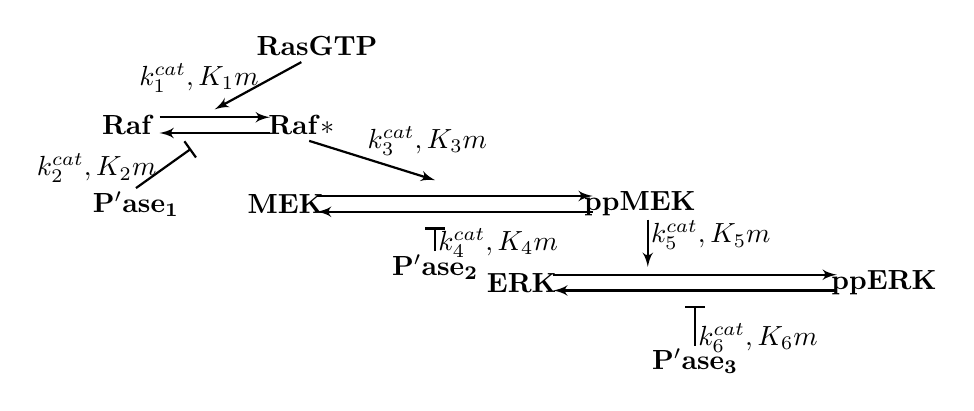
\begin{tikzpicture}[auto, outer sep=3pt, node distance=2cm,>=latex']

\node  at (-5.7, 9) (X3) {$\bf Ras \mhyphen GTP$};
\draw [->, thick] (-5.9, 8.8) ->  (-7, 8.2);
\node  at (-7.2, 8.6) (X3) {$k_1^{cat},K_1m$};


\node  at (-8.1, 8) (XGDP) {$\bf Raf$};
\draw [->, thick] (-7.7, 8.1) ->  (-6.3, 8.1);
\draw [<-, thick] (-7.7, 7.9) ->  (-6.3, 7.9);
\node  at (-5.9, 8) (XGDP) {$\bf Raf*$};

\node  at (-8, 7) (XGDP) {$\bf P'ase_1$};
\draw [-|, thick] (-8, 7.2) ->  (-7.3, 7.7);
\node  at (-8.5, 7.45) (X3) {$k_2^{cat},K_2m$};


%\draw [->, thick] (-5.8, 7.8) ->  (-5, 7.3);
\draw [->, thick] (-5.8, 7.8) ->  (-4.2, 7.3);

%\node  at (-6.1, 7.45) (X3) {$k_3^{cat},K_3m$};
\node  at (-4.3, 7.8) (X3) {$k_3^{cat},K_3m$};

\node  at (-6.1, 7) (XGDP) {$\bf MEK$};
\draw [->, thick] (-5.7, 7.1) ->  (-2.2, 7.1);
\draw [<-, thick] (-5.7, 6.9) ->  (-2.2, 6.9);
%\node  at (-3.9, 7) (XGDP) {$\bf p \mhyphen MEK$};
%\draw [->, thick] (-3.4, 7.1) ->  (-2.2, 7.1);
%\draw [<-, thick] (-3.4, 6.9) ->  (-2.2, 6.9);
\node  at (-1.6, 7) (XGDP) {$\bf pp \mhyphen MEK$};

\draw [->, thick] (-1.5, 6.8) ->  (-1.5,   6.2);
%\draw [->, thick] (-1.5, 6.8) ->  (0.2, 6.2);

\node  at (-4.2, 6.2) (XGDP) {$\bf P'ase_2$};
%\draw [-|, thick] (-6, 6.2) ->  (-5, 6.7);
\draw [-|, thick] (-4.2, 6.4) ->  (-4.2, 6.7);

\node  at (-3.4, 6.5) (X3) {$k_4^{cat},K_4m$};
%\node  at (-4.3, 6.2) (X3) {$k_6^{cat},K_6m$};


\node  at (-3.1, 6) (XGDP) {$\bf ERK$};
\draw [->, thick] (-2.7, 6.1) ->  (0.9, 6.1);
\draw [<-, thick] (-2.7, 5.9) ->  (0.9, 5.9);
%\node  at (-0.9, 6) (XGDP) {$\bf p \mhyphen ERK$};
%\draw [->, thick] (-0.4, 6.1) ->  (0.9, 6.1);
%\draw [<-, thick] (-0.4, 5.9) ->  (0.9, 5.9);
\node  at (1.5, 6) (XGDP) {$\bf pp\mhyphen ERK$};

%\node  at (-2.3, 6.4) (X3) {$k_7^{cat},K_7m$};
\node  at (-0.7, 6.6) (X3) {$k_5^{cat},K_5m$};


\node  at (-0.9, 5) (XGDP) {$\bf P'ase_3$};
\draw [-|, thick] (-0.9, 5.2) ->  (-0.9, 5.7);

\node  at (-0.1, 5.3) (X3) {$k_{6}^{cat},K_{6}m$};


%\draw [thick] (1.5, 5.75) --  (1.5, 3.9);
%\draw [thick] (1.5, 3.9) --  (-7.05, 3.9);
%\draw [-|, thick] (-7.05, 3.9) --  (-7.05, 7.7);

%\node  at (-3, 4.15) (X3) {$k_{7}^{cat},K_{7}m$};

\end{tikzpicture}
} }

\end{document}

